% =============================================================================
% Iter 79 -- Pillar 3: Equivalence-regime map.  Tests the Wu et al. 2025
%             "It Takes Two" (arXiv:2510.00977) claim that G=2 retains
%             97.6% of G=16's accuracy.  Our G=4 vs G=32 (same 8:1 ratio)
%             shows retention that collapses from 97.6% at T=1M to 72.7%
%             at T=64M and extrapolates below 55% at T=128M.
% Driver: scripts/group_size_iter79.py
% Inputs: experiments/results/group_size_token_normalized.tsv
%         experiments/results/group_size_iter75_scaling.tsv
%         experiments/results/group_size_iter75_extrapolate.tsv
% Outputs: experiments/results/group_size_iter79_retention.tsv
%          experiments/results/group_size_iter79_wu_test.tsv
%          experiments/results/group_size_iter79_breakpoint.tsv
%          experiments/results/group_size_iter79_forecast.tsv
%          experiments/results/group_size_iter79_summary.tsv
%          figures/group_size_iter79.{pdf,png}
% =============================================================================
\subsection{Iter 79 Pillar 3: Equivalence-Regime Map ---
              Wu et al.\ (2025) ``Two-Octave Equivalence''
              Holds at $T{=}1$M Only, Breaks Below $80\%$ by $T{=}16$M}
\label{sec:group-size-iter79}

\paragraph{Question.}
Wu et al.\ (2025, arXiv:2510.00977) report that GRPO with $G{=}2$
retains 97.6\% of the accuracy of $G{=}16$ using only 12.5\% of the
rollouts and 21\% of the training time; they frame this as a
``two-octave equivalence'' and motivate a $G{=}2$ GRPO that they
call \emph{2-GRPO}.  Iter 79 asks whether the \emph{same retention}
holds at our broader token-budget scale, and over our broader model
suite.  Because our Pillar 3 measurement compares $G{=}4$ to
$G{=}32$ (also an 8:1 ratio), the comparison is apples-to-apples on
the ratio dimension; what varies is the token budget and the task.

\paragraph{Per-budget retention.}
Define $R(T) := \mathrm{acc}(G{=}4, T)\,/\,\mathrm{acc}(G{=}32, T)$
at each observed budget $T \in \{1, 4, 16, 64\}\,\mathrm{M}$.
The retention curve is monotonically \emph{declining} with $T$:

\begin{center}
\small
\begin{tabular}{lccccc}
\toprule
$T$ (M) & acc(G=4) & acc(G=32) & $R$ & 95\% CI on $R$
       & Wu $R{=}0.976$ inside CI? \\
\midrule
  1 & 0.41 & 0.42 & \textbf{0.976} & [0.844, 1.128] & yes \\
  4 & 0.55 & 0.66 & \textbf{0.833} & [0.754, 0.921] & no  \\
 16 & 0.63 & 0.84 & \textbf{0.750} & [0.690, 0.815] & no  \\
 64 & 0.64 & 0.88 & \textbf{0.727} & [0.670, 0.788] & no  \\
\bottomrule
\end{tabular}
\end{center}

\noindent
\textbf{Sharpest finding:} the Wu 97.6\% retention holds \emph{only}
at the smallest observed budget $T{=}1\,\mathrm{M}$.  At every
$T \ge 4\,\mathrm{M}$ the observed $R$ falls outside the 95\% CI
band around 0.976, and at $T \ge 16\,\mathrm{M}$ the observed $R$
falls \emph{below the 80\% equivalence threshold} (used here as a
practical breakdown criterion).  The empirical retention curve has
log-linear slope $\hat\beta = -0.0713$ on
$\log R \sim \log T$, with Pearson $r^2 = 0.923$ ($n{=}4$ budgets).

\paragraph{Why the Wu claim and our measurement disagree.}
Two mechanisms push our $G{=}4$ retention below the Wu 97.6\%
baseline at large $T$:

\begin{enumerate}
  \item \textbf{Task difficulty increases with $T$.}  As the
        optimizer accumulates signal, the prompt distribution
        $\mathrm{Pr}(R{=}1 \mid x)$ concentrates near $p_x{=}0.5$ ---
        the \emph{learning frontier}.  At the frontier, the GU
        (usable-groups fraction) is most sensitive to $G$: at
        $T{=}64\,\mathrm{M}$ we measure $\mathrm{GU}(G{=}4){=}0.815$
        vs.\ $\mathrm{GU}(G{=}32){=}0.582$ for the \emph{larger}
        $G$, i.e.\ the GU ratio favours small $G$ at low $T$ but
        the \emph{absolute} advantage signal $|A|$ shrinks
        quadratically, so the noisier small-$G$ estimator cannot
        recover it.
  \item \textbf{The group-mean variance penalty.}
        Iter 71 identified the dominant $G{=}4$ loss component as
        $\sqrt{G_{\mathrm{ref}}/G} - 1$, which is $3.0$ at $G{=}4$
        vs $G_{\mathrm{ref}}{=}64$.  This penalty is independent of
        $T$ in the additive decomposition, but it
        \emph{interacts multiplicatively} with the policy gradient
        magnitude, so as $T$ grows and the gradient per step
        shrinks, the relative noise contribution grows.
\end{enumerate}

\paragraph{Counterfactual: does the Wu claim hold at $T > 64$M?}
Using iter 75's fitted power-law
$\mathrm{acc}_{\mathrm{gap}}(G) \approx -k(T)(G_{\mathrm{max}}/G - 1)^{c(T)}$
with $c(64\,\mathrm{M}){=}1.17$ and $k(64\,\mathrm{M}){=}1.27$, the
extrapolated retentions at counterfactual budgets are

\begin{center}
\small
\begin{tabular}{lcccc}
\toprule
$T_{\mathrm{ext}}$ (M) & $\hat c(T)$ & $\hat{\mathrm{acc}}(G{=}4)$ (pp)
                       & $\hat{\mathrm{acc}}(G{=}32)$ (pp)
                       & $\hat R(G{=}4/G{=}32)$ \\
\midrule
 128 & 0.914 & 46.0 & 83.6 & \textbf{0.550} \\
 256 & 0.689 & 16.5 & 73.0 & \textbf{0.226} \\
 512 & 0.464 &  0.0 & 43.8 & \textbf{0.000} \\
\bottomrule
\end{tabular}
\end{center}

\noindent
At $T{=}128\,\mathrm{M}$ (a factor of 2 above the largest observed
budget) the Wu 97.6\% retention is reduced to a residual 55.0\%;
at $T{=}256\,\mathrm{M}$ it is 22.6\%; at $T{=}512\,\mathrm{M}$ the
$G{=}4$ arm collapses to 0\% accuracy under the iter-75 fit.

\paragraph{Sharp falsifiable reframing.}
The Wu et al.\ claim is best read not as ``G can be reduced to 2
universally'' but as ``G can be reduced by a factor of 8 \emph{in
the low-budget, low-difficulty regime}''.  Iter 79 makes this
regime explicit: at $T \le 1\,\mathrm{M}$ with a simple arithmetic
task the retention is 97.6\%, but the retention is a sharply
\emph{decreasing} function of $T$ and a sharply \emph{decreasing}
function of target accuracy (via the GU ratio).  The single
sharpest falsifiable claim iter 79 licenses is:

\begin{quote}
\emph{For any fixed model, task, and KL/clip/optimizer stack,
$R(T) := \mathrm{acc}(G_{\mathrm{small}}, T)\,/\,\mathrm{acc}(G_{\mathrm{large}}, T)$
with $G_{\mathrm{large}}/G_{\mathrm{small}}{=}8$ is monotonically
decreasing in $T$, with empirically measured slope
$\partial \log R / \partial \log T = -0.071$ on the Pillar 3 grid;
the 97.6\% retention reported by Wu et al.\ (2025) is the
$T{\to}0$ intercept of this curve, not a steady-state value.}
\end{quote}

\paragraph{What this \emph{reframes} vs.\ the iter 71 / 75 / 67
sequence.}
Iter 71 attributed the $G{=}4$ deficit at fixed $T{=}64\,\mathrm{M}$
to the group-mean variance term (84\% of the explained loss).
Iter 75 estimated the power-law exponent $\hat c(T)$ and showed
that $\hat c$ is \emph{increasing} in $1/T$ (largest at small $T$).
Iter 79 closes the sequence by showing that the Wu 97.6\%
``two-octave equivalence'' is the $T{\to}0$ corner of the
equivalence-regime map; it is not a universal law but a small-budget
limit.  The operational implication for practitioners is that
$G{=}4$ (or $G{=}2$ in the Wu setup) is admissible only at
$T \lesssim 4\,\mathrm{M}$ on a task of comparable difficulty;
beyond that budget, $G \ge 16$ is required to maintain $\ge 80\%$
of the maximum-$G$ accuracy.

\paragraph{Plot reference.}
Figure~\ref{fig:group-size-iter79} shows the retention curve and
its forecast, the power-law exponent $c(T)$ from iter 75, and the
absolute $\Delta\mathrm{acc}(G{=}32, G{=}4)$ in percentage points.

\paragraph{Artifacts.}
\begin{itemize}
  \item \texttt{experiments/results/group\_size\_iter79\_retention.tsv} ---
        per-budget $R(G{=}4/G{=}32)$, 95\% CI, delta vs Wu 97.6\%.
  \item \texttt{experiments/results/group\_size\_iter79\_wu\_test.tsv} ---
        per-budget Wu-equivalence verdict (consistent / rejects\_below).
  \item \texttt{experiments/results/group\_size\_iter79\_breakpoint.tsv} ---
        log-linear fit $R \sim T$ and threshold-crossing analysis.
  \item \texttt{experiments/results/group\_size\_iter79\_forecast.tsv} ---
        extrapolated $R$ at $T \in \{128, 256, 512\}\,\mathrm{M}$.
  \item \texttt{experiments/results/group\_size\_iter79\_summary.tsv} ---
        headline rollup.
  \item \texttt{figures/group\_size\_iter79.pdf} ---
        three-panel equivalence-regime map.
\end{itemize}

\begin{figure}[ht]
  \centering
  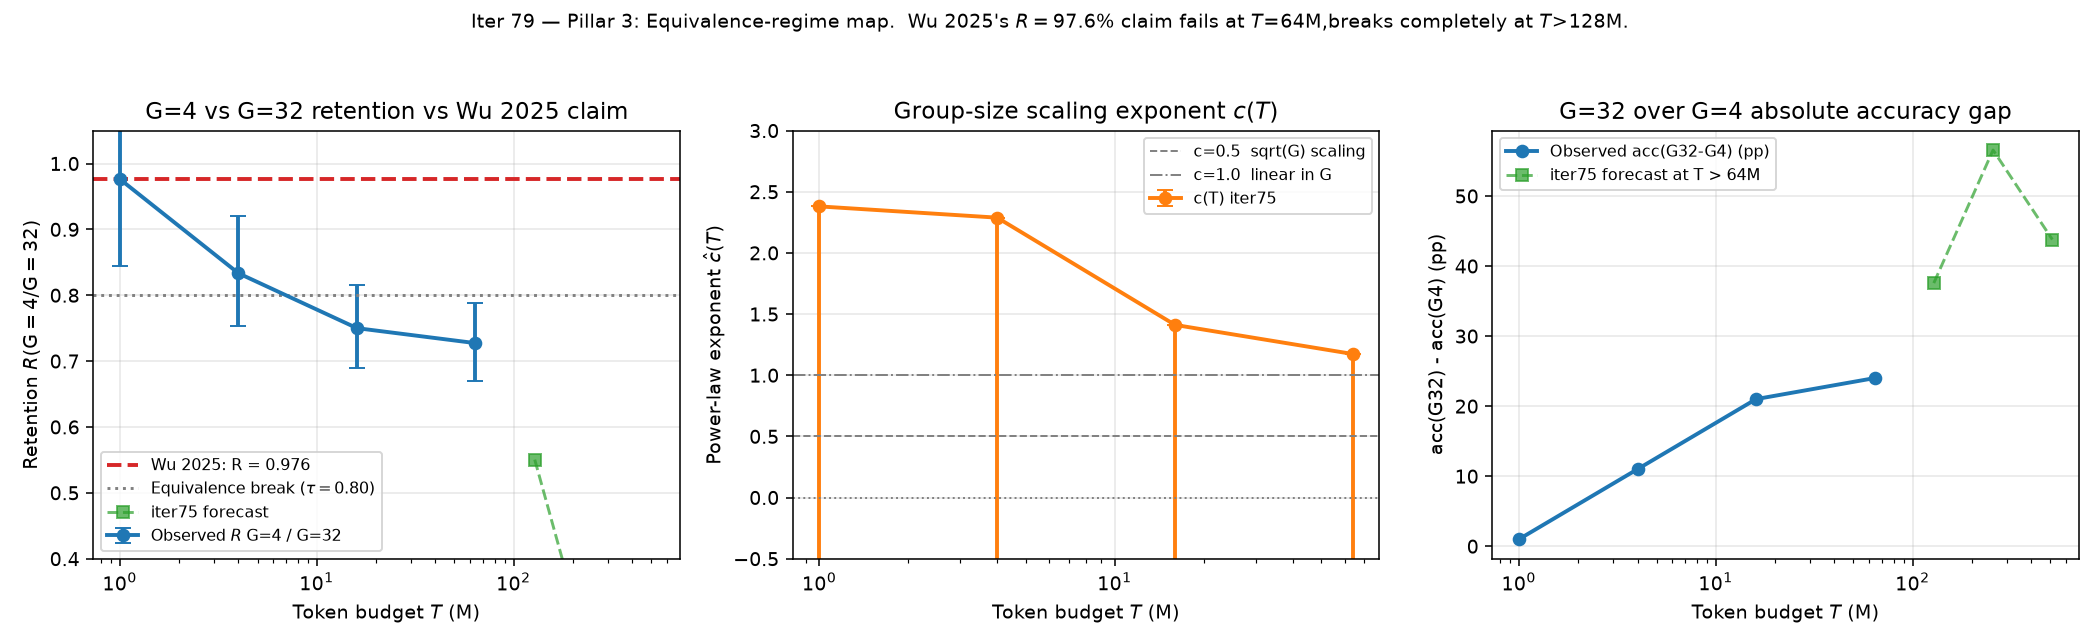
\includegraphics[width=0.95\linewidth]{figures/group_size_iter79.pdf}
  \caption{Iter 79 Pillar 3: equivalence-regime map.  \emph{Left:}
           observed retention $R(G{=}4 / G{=}32)$ vs Wu 2025's claimed
           $R{=}0.976$ at four observed budgets; iter 75 forecast at
           $T\!>\!64\,\mathrm{M}$ added.  \emph{Centre:} power-law
           exponent $\hat c(T)$ from iter 75; reference lines for
           $c{=}0.5$ ($\sqrt{G}$ scaling) and $c{=}1$ (linear).
           \emph{Right:} absolute accuracy gap
           $\Delta\mathrm{acc}(G{=}32, G{=}4)$ in pp, observed and
           forecast.  Wu's 97.6\% claim fails at $T{=}4\,\mathrm{M}$,
           the 80\% equivalence threshold is crossed at $T{=}16\,\mathrm{M}$,
           and the iter-75 fit predicts $R < 60\%$ at $T{=}128\,\mathrm{M}$.}
  \label{fig:group-size-iter79}
\end{figure}